\chapter{Analisis dan Perancangan}

\section{Analisis Permasalahan}
Untuk mencapai tujuan pada pada subbab I.3, tedapat tiga komponen permasalahan: infeksi malware, deteksi malware dan penangkalan infeksi.

\subsection{Infeksi Malware}
Dalam penelitian ini, sebuah host disebut terinfeksi oleh malware jika sebuah perilaku malicious dari malware dilakukan oleh host tersebut. Host dapat berupa skala mesin komputer atau sebuah executable. Berbeda dengan \textit{compromised host} yang berarti ketika \textit{attacker} mendapatkan akses terhadap host. Infeksi malware berbeda untuk masing-masing jenis malware. Dalam analisis ini dan analisis selanjutnya akan dilakukan dalam klasifikasi worm, virus dan bot. Klasifikasi ini dilakukan dari sudut pandang bagaimana malware dapat dideteksi dan bagaimana malware menyembunyikan diri.

\subsubsection{Infeksi Virus}

Infeksi oleh virus dilakukan dengan cara menyisipkan kode ke executable lain (host). Bagian penting dari infeksi oleh malware kategori virus berada pada bagaimana virus menyembunyikan diri pada executable host. Beberapa cara menyembunyikan diri dari (\cite{6620049}) dan (\cite{alsamer2016}) yakni: \textit{obfuscation}, enkripsi, \textit{oligomorphic}, \textit{polymorphic}, \textit{metamorphic}.

Teknik \textit{obfuscation} dilakukan dengan cara menambahkan perintah \textit{garbage} kedalam kode. Perintah \textit{garbage} dapat berupa perintah seperti nop pada assembly ataupun jump yang membuat kode virus terpotong-potong sehingga membuat signature menjadi lebih sulit didapatkan.

Selain itu beberapa virus menggunakan teknik enkripsi untuk mengodekan dirinya. Virus dengan jenis ini memiliki algoritma cipher, kunci, dan kode malicious yang terenkripsi. Teknik ini menjadikan virus dengan jenis ini kompleks. Setiap infeksi virus umunya dilakukan dengan mengubah kunci enkripsinya sehingga bagian kode malicious tidak dapat dijadikan sebagai signature. Namun karena terdapat algoritma \textit{cipher} yang sama, maka hal tersebut dapat menjadi signature.

\textit{Oligomorphic} merupakan teknik menyembunyikan diri dengan teknik enkripsi tetapi menggunakan algoritma cipher yang berubah dalam jangka waktu tertentu. Virus dengan jenis ini akan memiliki beberapa algoritma cipher yang dapat digunakan, dimana algoritma cipher akan berulang pada saat tertentu.

Sedangkan pada teknik \textit{polymorphic}, virus memiliki algoritma cipher yang tak terhingga banyaknya. Virus dengan jenis ini memiliki algoritma untuk membuat algoritma ciphernya secara acak. Sehingga untuk setiap infeksi, virus ini memiliki algoritma cipher baru dan kunci cipher baru.

Teknik \textit{metaphoric} merupakan teknik virus yang dapat menyebunyikan dirinya dalam bentuk lain yang tidak memiliki kemiripan dengan kode asalnya. Virus dengan jenis ini tidak memiliki algoritma cipher, namun untuk setiap infeksi kode dirinya berubah.

\subsubsection{Infeksi Worm}

Worm pada (\cite{alsamer2016}) disebut sebagai \textit{subclass} dari virus yang dapat hidup tersendiri. Worm memiliki karakteristik untuk dapat menyebarkan dirinya melalui jaringan dengan melakukan eksploit terhadap \textit{vulnerability} atau kesalahan pengaturan pada \textit{service} yang digunakan secara umum. Worm dapat dikategorikan menjadi dua kategori yakni: \textit{scan-based worm} dan \textit{topology-based worm}.

\textit{Scan-based worm} merupakan mencoba melakukan pemindaian lingkungan untuk dapat menginfeksi. Teknik pemindaian dapat berbentuk \textit{random scanning} atau \textit{localized scanning}. \textit{Random scanning} dilakukan dengan menemukan host secara acak yang dapat diinfeksi. Teknik untuk menemukan secara acak dapat menggunakan random number generator, list atau host yang dapat diakses melalui routing. \textit{Localized-scanning} dilakukan dengan cara menemukan host dalam linkungan yang tertentu untuk diinfeksi. \textit{Localized} yang dimaksud dapat berbentuk grup lokal yang memang ditarget oleh penyerang, atau jangkauan IP tertentu, atau secara melakukan pemindaian sekuensial dari IP. Localized-scanning dapat memperkecil waktu untuk penyebaran dibandingkan dengan random scanning karena malware memiliki pengetahuan tambahan dibanding \textit{random-scanning}.

\textit{Topology-based worm} melakukan infeksi dengan cara menemukan tetangga dari topologi yang dimiliki host. Jenis worm ini memiliki peluang yang berbeda untuk setiap usaha melakukan infeksinya. Penyebarannya memiliki karakteristik khusus, yakni memiliki \textit{user interference}. Peluang terjadinya \textit{user interference} berbeda-beda akibat beberapa faktor yang dimiliki oleh korban. Salah satu contoh \textit{user interference} yang dimanfaatkanz oleh worm kategori ini berupa email. Email digunakan oleh worm untuk mengirimkan salinannya misal dalam bentuk \textit{attachment}. Sehingga peluang penyebarannya akan bergantung pada faktor berapa sering korban membuka email dan membuka attachment.

\subsubsection{Infeksi Bot}

Hal yang perlu diperhatikan pada infeksi bot berada pada fase dan komponen malware ini. Menurut (\cite{alsamer2016}) fase pada malware kelas ini adalah: \textit{infection}, \textit{spreading}, \textit{rallying}, dan \textit{elusion}.

Pada fasa \textit{infection} malware pada umumnya dijalankan oleh penyerang pada sebuah host. Ketika host sudah terinfeksi, maka malware akan melanjutkan ke fasa selanjutnya, yaitu \textit{spreading}. Pada fasa \textit{spreading}, bot akan melakukan infeksi dapat berupa active maupun passive (\cite{alsamer2016}). Penyebaran secara aktif dilakukan dengan cara scanning seperti yang dilakukan oleh worm. Sedangkan penyebaran secara pasif dilakuakn dengan mengandalkan \textit{user inferference} yakni teknik seperti teknik topology yang digunakan pada worm.

Fasa \textit{rallying}, bot akan melakukan kontak dengan control server untuk mendapatkan perintah. Perintah dapat dikategorikan menjadi: pengintaian \textit{traffic}, \textit{denial of service}, \textit{compute power}, spam, dan menjadi saluran penyebaran malware. Untuk melakukan kontak dengan control server, malware dapat menggunakan IP, nama domain, ataupun menggunakan suatu algoritma yang dimiliki malware (\cite{alsamer2016}). Bagian ini merupakan bagian paling penting dalam malware kelas ini, karena bot tanpa adanya komunikasi dengan control server tidak memiliki tujuan (\cite{alsamer2016}). Selain itu bagian ini merupakan bagian yang paling mudah untuk dijadikan signature, misalnya dengan menemukan IP atau nama domain tertentu. Sehingga beberapa malware menggunakan teknik seperti IP flux atau DNS flux. Selain itu koneksi yang dilakukan dengan control server dapat menggunakan jaringan anonim, enkripsi, atau tunneling. 

Fasa ini juga bersamaan dengan fasa \textit{elusion}. Fasa \textit{elusion}, bot harus dapat menyembunyikan dirinya seperti mekanisme seperti \textit{polymorphism} yang dimiliki oleh kategori virus sehingga mempersulit signature dari bot untuk dikenali. 

\subsection{Deteksi Malware}

Menurut (\cite{6620049}), deteksi malware dikategorikan menjadi tiga, yakni: \textit{signature-based}, \textit{behavior-based}, dan \textit{heuristic-based}. \textit{Signature-based}, \textit{behavior-based}, dan \textit{Heuristic-based} pada (\cite{6620049}) dapat disamakan dengan \textit{static signature-based}, \textit{dynamic signature-based}, dan \textit{anomaly-based} berurutan pada (\cite{idika2007survey}). Dalam penelitian ini istilah yang digunakan mengacu pada (\cite{idika2007survey}).

Deteksi dengan menggunakan teknik \textit{anomaly-based detection} memiliki kelebihan dapat mendeteksi malware yang tidak dikenali. Namun deteksi dengan menggunakan teknik ini tidak dapat diaplikasikan secara praktis karena memiliki tingkat \textit{false-alarm} (\textit{false-positive}) yang tinggi. \textit{False-alarm} menjadi ancaman untuk availability sistem jika action dari rule melakukan disable terhadap sistem, ataupun koneksi.

Pada kasus malware dengan kelas virus, teknik-teknik seperti \textit{obfuscation}, enkripsi, \textit{oligomorphic}, \textit{polymorphic}, dan \textit{metamorphic} menjadikan deteksi dengan menggunakan static signature-based menjadi lebih sulit dilakukan. Seperti yang telah dibahas sebelumnya, pada teknik obfuscation masih dimungkinkan untuk mendapatkan signature berupa potongan kode malware. Kemudian pada teknik enkripsi dapat dideteksi dengan menemukan signature berupa algoritma cipher yang digunakan. Pada oligomorphic masih dapat dilakukan dengan menemukan sejumlah himpunan algoritma enkripsi yang digunakan malware. Namun pada polymorphic atau methamorphic dengan teknik deteksi static signature-based menjadi lebih rumit untuk dilakukan.

Implementasi \textit{dynamic signature-based} menurut (\cite{6620049}) memiliki tiga komponen utama, yakni: \textit{data collector}, \textit{interpreter}, dan \textit{matcher}. Komponen \textit{data collector} menjadi bagian yang mengumpulkan informasi perilaku yang dilakukan oleh \textit{executable}. \textit{Interpreter} menjadi komponen yang menjadi perantara untuk memproses informasi yang telah dikumpukan menjadi informasi yang dapat digunakan oleh matcher. Kemudian \textit{matcher} menentukan apakah sebuah executable dideteksi sebagai malware.

Pada kasus malware dengan kelas worm, seperti yang telah dijelaskan pada subbab sebelumnya merupakan subkelas dari virus. Deteksi dengan menggunakan \textit{static signature-based} akan rumit ketika malware menggunakan teknik \textit{polymorphic} atau \textit{metamorphic}. Deteksi worm dengan menggunakan dynamic signature-based mungkin untuk dilakukan pada skala host. \textit{Dynamic signature-based} dapat dilakukan generalisasi tidak hanya untuk mendeteksi malware dalam bentuk \textit{executable}. Struktur komponen \textit{data collector}, \textit{interpreter}, dan \textit{matcher} pada dynamic signature-based dapat digeneralisasi untuk host ataupun sebuah sistem. Jadi, deteksi dengan teknik ini dapat digunakan untuk menentukan apakah sebuah host (mesin) telah terinfeksi, atau juga dapat digunakan dalan bentuk sistem. Seperti yang dilakukan oleh IDS untuk mendeteksi infeksi pada skala host.

Deteksi dengan \textit{dynamic signature-based} dapati digolongkan menjadi dua stateful dan stateless detection. Pada stateless detection, matcher menentukan sebuah host atau executable malicious hanya menggunakan informasi yang diberikan oleh interpreter tanpa menyimpan state. Deteksi stateless ini dapat melakukan deteksi yang hemat sumber-daya. Namun, deteksi ini tidak dapat menemukan \textit{behavior} yang rumit dari sebuah malware. Sedangkan deteksi stateful dynamic signature-based, menentukan sebuah host atau executable malicious dengan menggunakan state yang disimpan oleh matcher. Namun, deteksi jenis ini membutuhkan lebih banyak sumber-daya.

\subsubsection{Stateful dynamic signature-based detection}

\textit{Stateful dynamic signature-based detection} dapat direpresentasikan menggunakan state machine. State machine secara matematis dapat dimodelkan sebagai quintuple ($\Sigma$, $S$, $s_0$, $\delta$, $F$). $\Sigma$ sebagai himpunan alfabet input, $S$ sebagai himpunan state, $s_0$ sebagai state awal, $F$ sebagai himpunan state akhir, dan $\delta$ sebagai fungsi transisi yang memetakan $\delta : S \times \Sigma \rightarrow S$. 

Dalam deteksi penyebaran worm dalam jaringan menggunakan \textit{stateful dynamic signature-based detection} dapat menggunakan beberapa kategori state machine: \textit{connection-based state machine}, \textit{sender-based state machine}, \textit{target-based state machine}, \textit{pair-based state machine}.

Pada \textit{connection-based state machine}, State machine \textit{connection-based} memiliki ciri $s_0$ berupa state awal koneksi terbentuk, dan $\Sigma$ merupakan himpunan paket-paket signature dalam koneksi tersebut. State machine dengan jenis ini dapat diterapkan untuk mendeteksi pada malware yang melakukan infeksi dalam satu buah koneksi.

Pada \textit{sender-based state machine}, $\Sigma$ merupakan himpunan paket signature yang dikirim dari sebuah host. $s_0$ dapat berupa state ketika sebuah host mulai terlihat aktif dari sisi detector, atau ketika detector baru diaktifkan seluruh host akan memiliki state ini. State machine ini dapat digunakan untuk mendeteksi host yang melakukan aktivitas malicious sehingga bisa dijadikan alarm ketika host terinfeksi.

\textit{Target-based state machine} sedikit berbeda dengan \textit{sender-based state machine}, $\Sigma$ merupakan himpunan paket signature yang diterima dari sebuah host. State machine ini dapat digunakan untuk mendeteksi ketika sebuah host diserang oleh beberapa host dengan pola tertentu. Namun state machine ini tidak memiliki state host yang melakukan serangan.

Pada \textit{$N$-tuple-based state machine}, $\Sigma$ merupakan himpunan yang paket signature pada komunikasi $N$-host. Jenis ini dapat mendeteksi ketika sebuah host diserang oleh beberapa host dengan pola tertentu, dan menyimpan state dari host mana serangan dilakukan. State machine ini lebih kompleks dari \textit{target-based state machine}.

\subsection{Penangkalan Infeksi Malware}

Proses penangkalan infeksi malware dapat dilakukan ketika deteksi telah dilakukan dan mendapatkan hasil positif. Untuk melakukan penangkalan infeksi malware, dapat dilakukan target-drop, sender-drop, atau connection-drop. Teknik target-drop dan sender-drop dapat dilakukan ketika sebuah host diindikasi diserang atau menyerang. Teknik ini dapat digunakan untuk mencegah infeksi meluas. Namun, teknik ini dapat mengganggu availability service dan teknik ini jarang ditemui dalam penerapan. Connection-drop merupakan teknik yang menghalangi koneksi terjadi ketika indikasi serangan ditemukan. Teknik ini merupakan teknik yang digunakan pada firewall.

\section{Analisis Batasan Permasalahan}

Pada bagian ini, penulis melakukan analisis untuk mendapatkan signature dari malware WannaCry, yang menjadi batasan masalah. Metodologi yang penulis lakukan sebagai berikut:

\begin{enumerate}
	\item {Melakukan studi literatur vulnerability yang dieksploit oleh malware;}
	\item {Melakukan packet capture packet yang dikirim oleh malware;}
	\item {Analisis hasil packet capture terhadap studi literatur}
\end{enumerate}

Packet capture pada lalu lintas paket malware WannaCry dilakukan dengan melakukan \textit{sniffing} dengan menggunakan 3 host dengan jaringan terisolasi seperti pada gambar \ref{fig:analisis_malware_net}.

\begin{figure}[H]
	\centering
	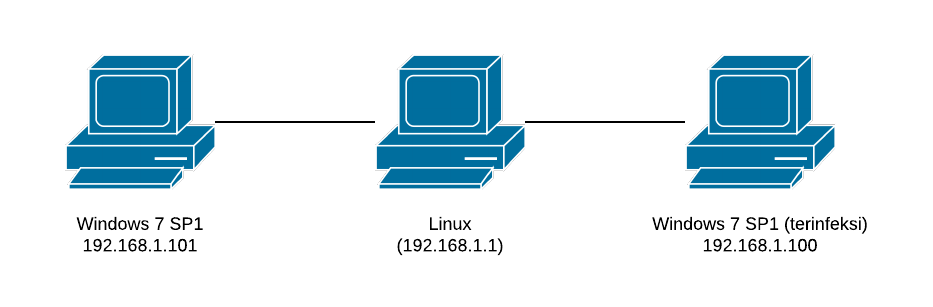
\includegraphics[width=400px]{resources/analisis_malware_net.png}
	\caption{Susunan jaringan untuk analisis malware WannaCry}
	\label{fig:analisis_malware_net}
\end{figure}

Host linux (192.168.1.1) merupakan host dengan dua interface yang difungsikan sebagai \textit{bridge}. Sehingga host Windows 7 terinfeksi (192.168.1.100) dapat berkomunikasi dengan host Windows 7 (192.168.1.101) hanya melalui 192.168.1.1. Kemudian pada host linux dilakukan sniffing dengan menggunakan tcpdump. dengan command sebagai berikut:

\begin{verbatim}
$ tcpdump -s0 -i br0 -vv -w output.wannacry-1.pcap
\end{verbatim}

\subsubsection{Hasil Studi Literatur}

Dari riset yang telah dilakukan oleh \cite{islam2018smb}, WannaCry melakukan exploit terhadap vulnerability EternalBlue dan DoublePulsar yang ada pada implementasi SMB1. EternalBlue merupakan vulnerability yang diakibatkan oleh 3 buah bug yang menurut (\cite{islam2018smb}) dan (\cite{grossman2017check}) yakni:
\begin{enumerate}
	\item Wrong casting bug
	\item Wrong parsing function bug
	\item Non-paged pool allocation bug
\end{enumerate}

Paket yang dikirimkan malware untuk mengeksploitasi vulnerability (\cite{islam2018smb}) yakni dengan mengirimkan \verb|SMB_COM_NT_TRANSACT|  diikuti dengan \verb|SMB_COM_TRANSACTION2_SECONDARY|.

\subsubsection{Analisis Hasil Packet Capture}

Berdasarkan pengelompokan malware menjadi worm, virus, dan trojan horse; WannaCry digolongkan sebagai worm. Sesuai dengan karakteristik yang disebutkan dalam dasar teori, WannaCry memiliki kapabilitas menginfeksi melalui network.

WannaCry memiliki dua buah bagian utama: ransomware, dan worm penginfeksi, yang melakukan penyebaran melalui protokol SMB. Jika sebuah host hanya menjalankan bagian ransomware saja, maka tidak akan ada penyebaran yang dilakukan, seperti ditunjukan pada Gambar \ref{fig:no_infect_action}. Sedangkan jika host menjalankan bagian dropper, dropper tersebut akan menjalankan worm penginfeksi dan sekaligus menjalankan ransomware. Pada Gambar \ref{fig:infect_action} terlihat host 192.168.1.100  mencoba melakukan koneksi ke port \verb|445/tcp| setiap host yang berada pada subnet yang sama.

\begin{figure}[H]
	\centering
	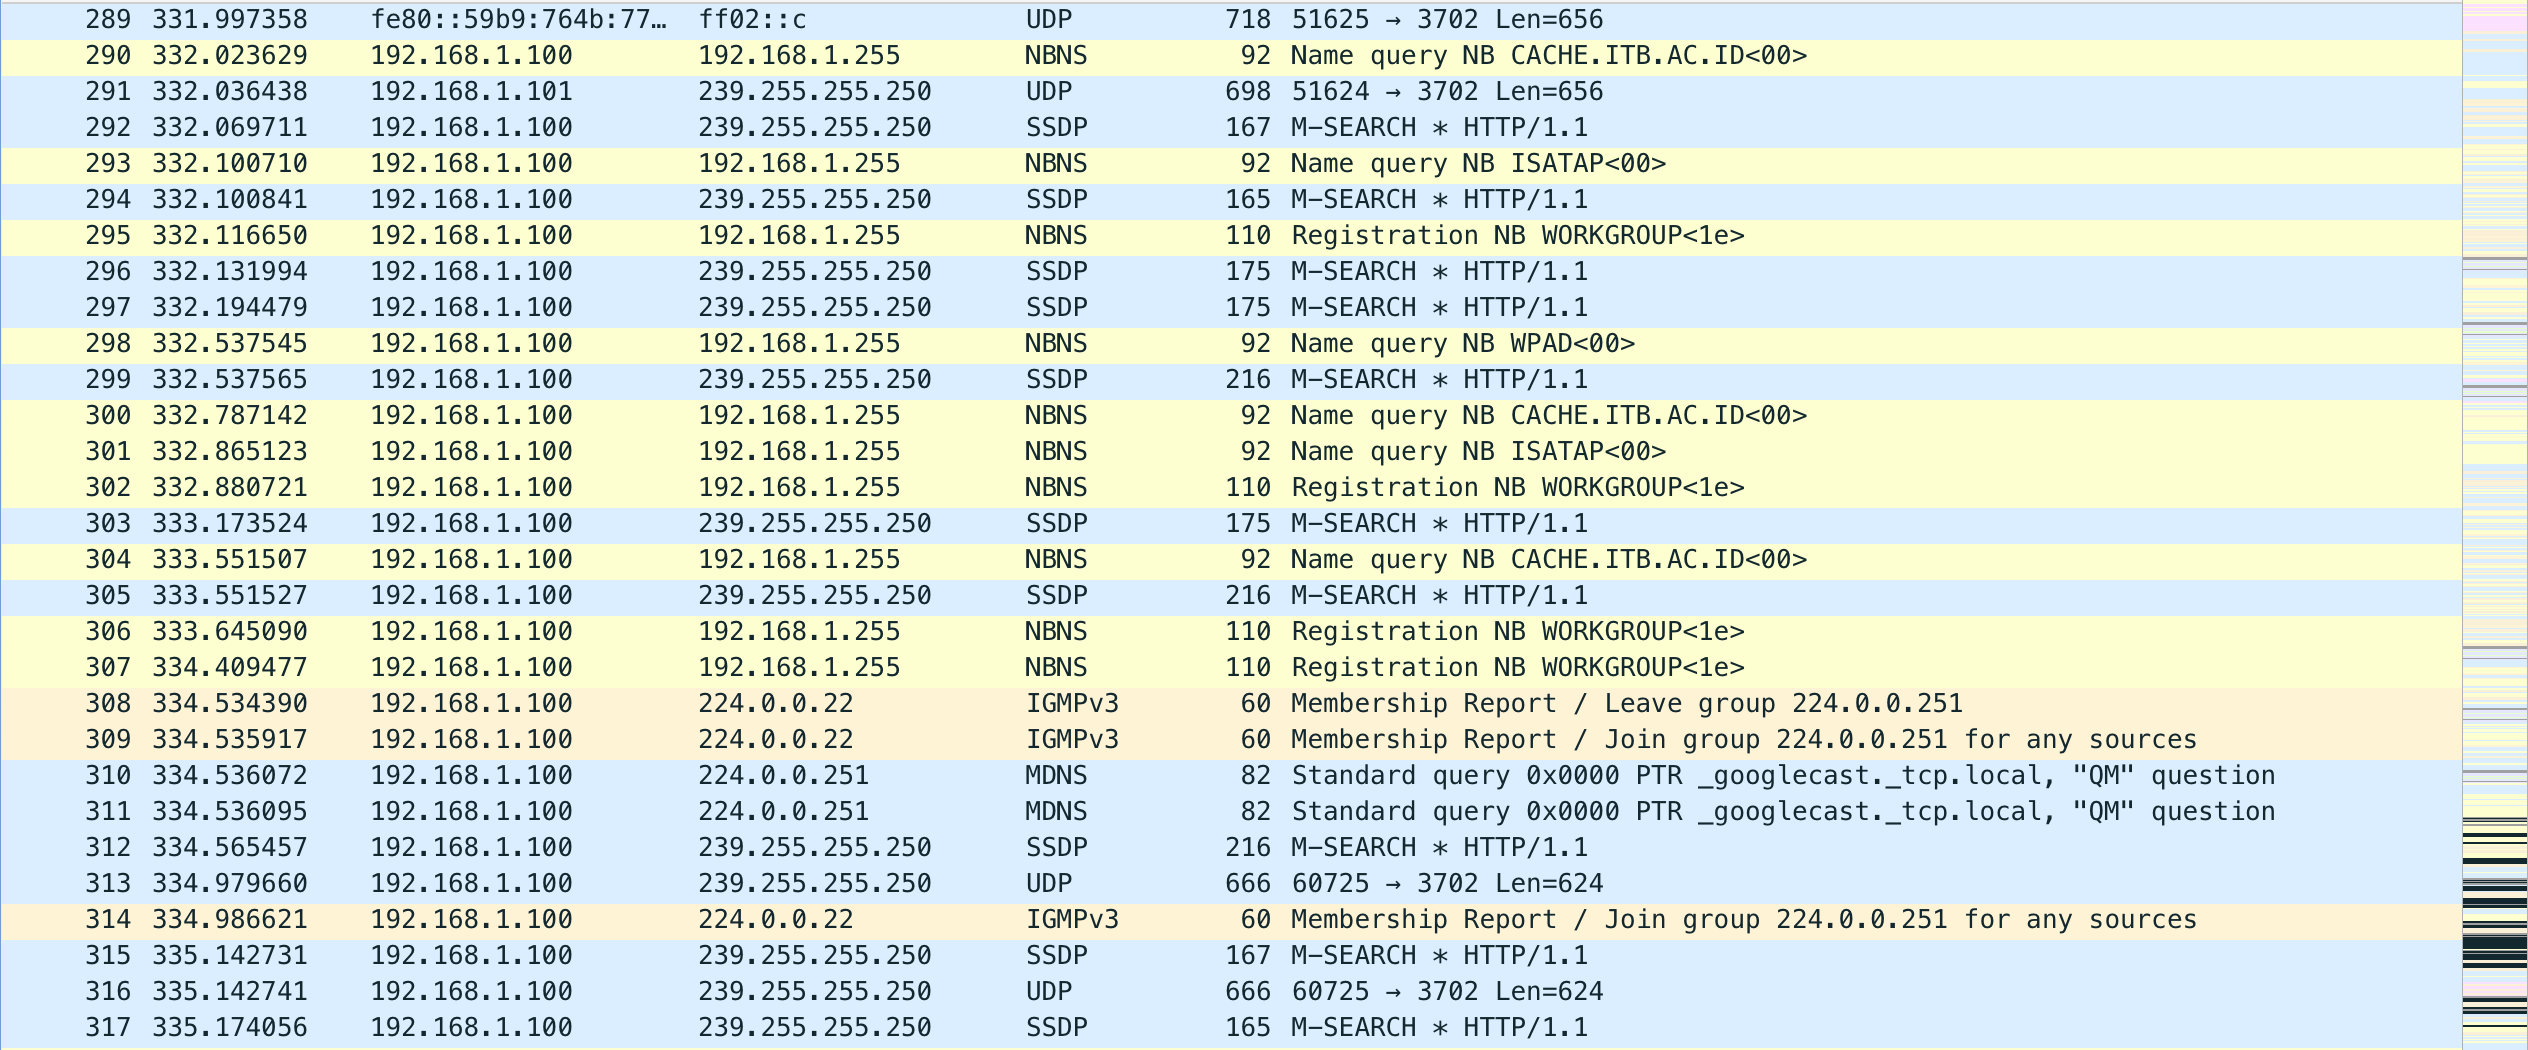
\includegraphics[width=\textwidth]{resources/no_infect_action.png}
	\caption{Paket pada host terinfeksi ransomware tanpa worm penginfeksi}
	\label{fig:no_infect_action}
\end{figure}

\begin{figure}[H]
	\centering
	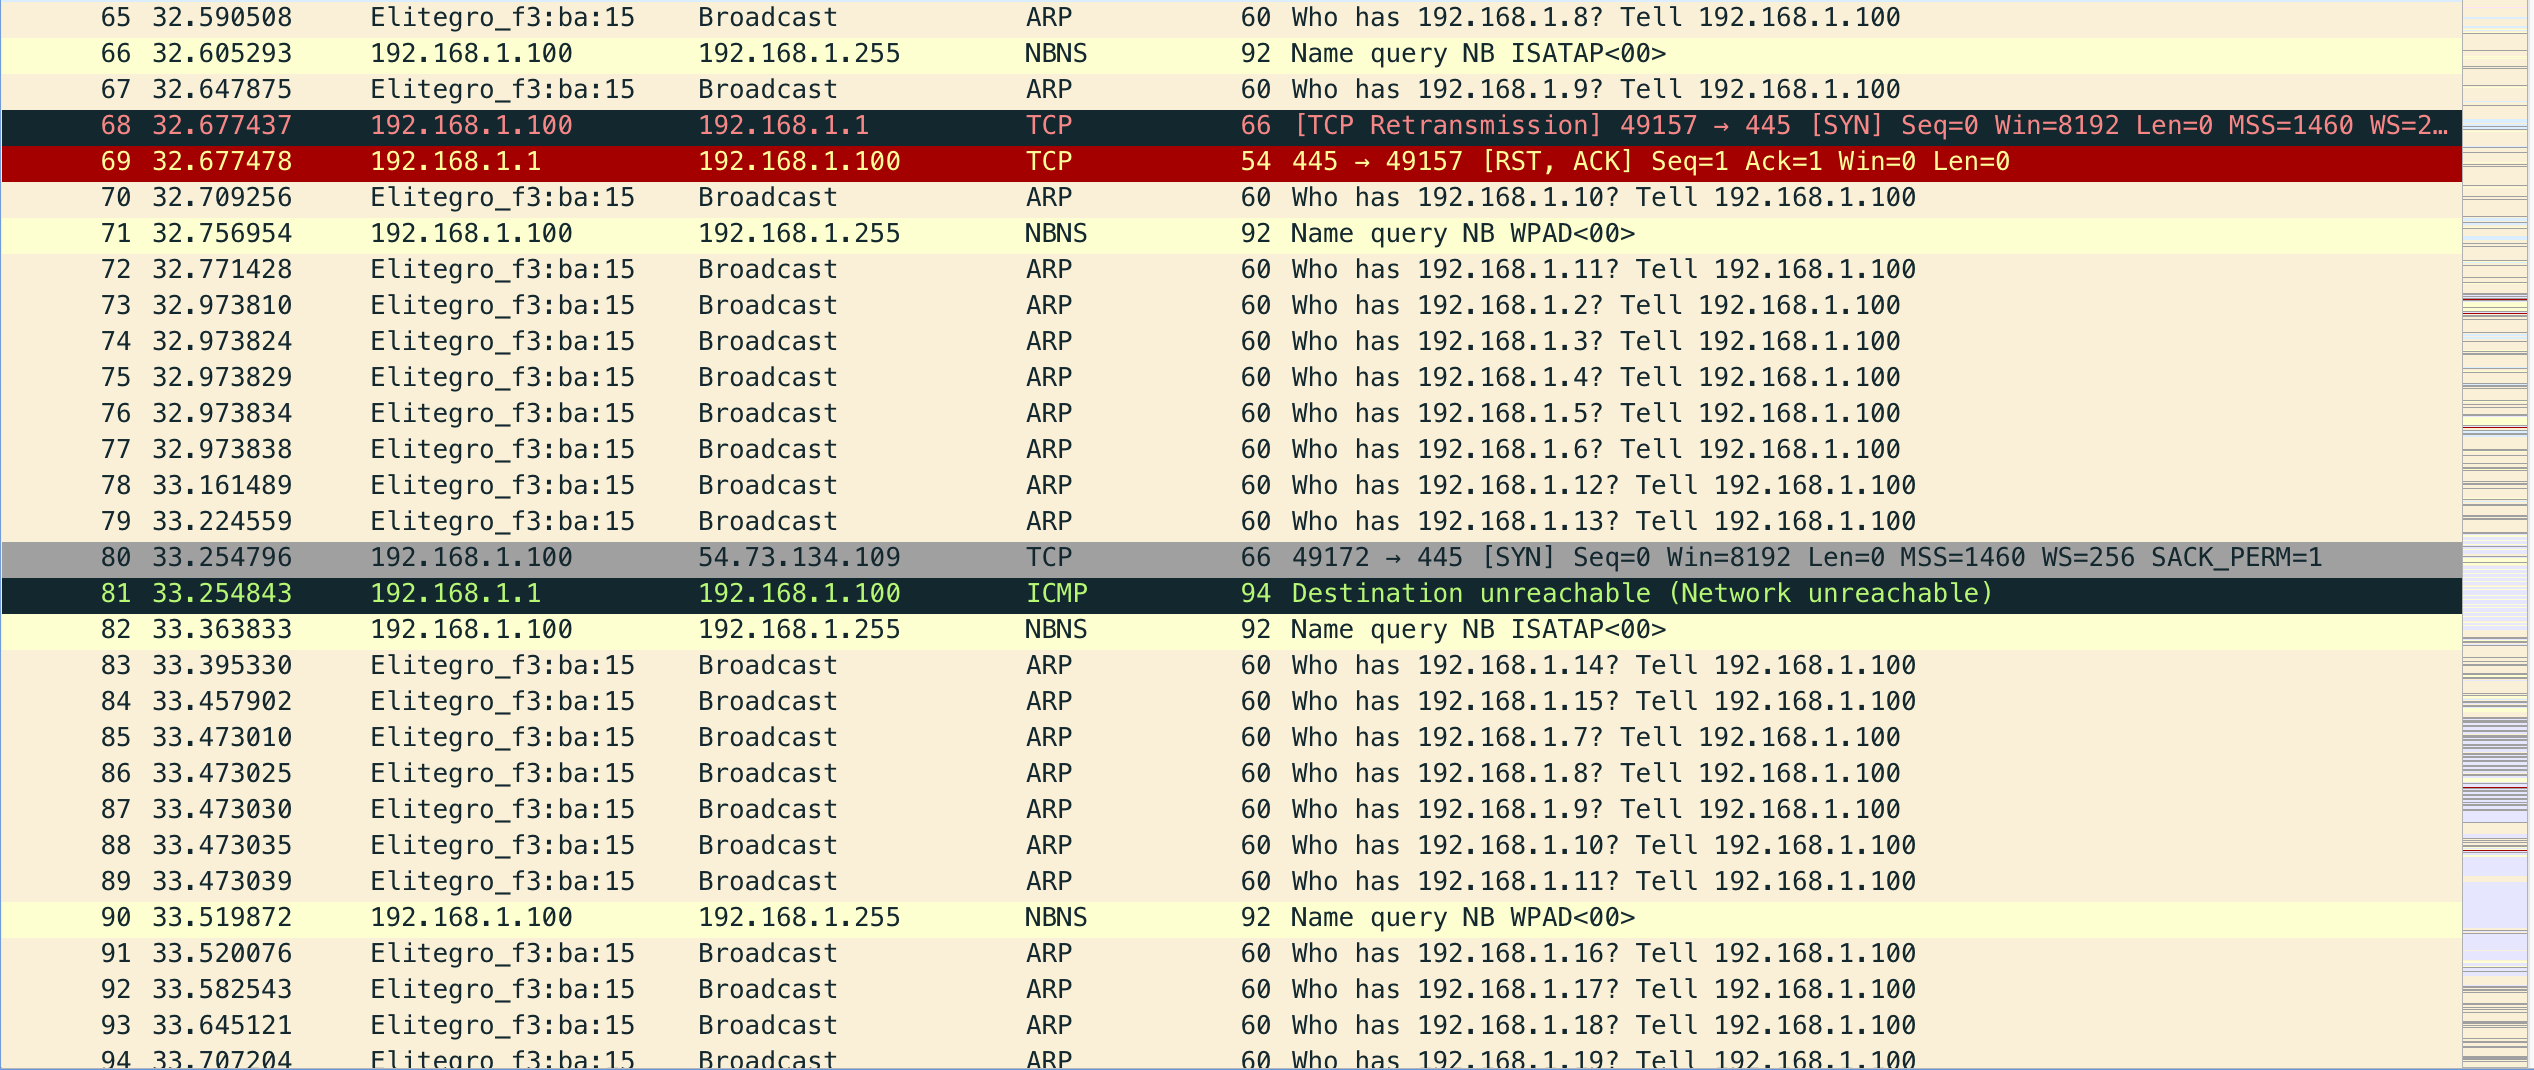
\includegraphics[width=\textwidth]{resources/infect_action.png}
	\caption{Paket pada host terinfeksi ransomware dengan dropper}
	\label{fig:infect_action}
\end{figure}

Ransomware merupakan kategori malicious software yang ketika dijalankan akan menonaktifkan fungsi tertentu dari komputer dengan sebuah cara. Kemudian ransomware akan menampilkan pesan untuk meminta pembayaran untuk mengembalikan fungsi yang dinonatifkan. Sehingga malware seakan-akan melakukan penyandraan terhadap komputer. (\cite{o2012ransomware}).

Pada paket yang dikirimkan host 192.168.1.100 terlihat malware berusaha mengeksploitasi vulnerability seperti yang disebutkan (\cite{islam2018smb}), yakni dengan mengirimkan \verb|SMB_COM_NT_TRANSACT| terlihat pada Gambar \ref{fig:trans_nop}, diikuti dengan \verb|SMB_COM_TRANSACTION2_SECONDARY| seperti pada Gambar \ref{fig:trans2_secondary}.

\begin{figure}[H]
	\centering
	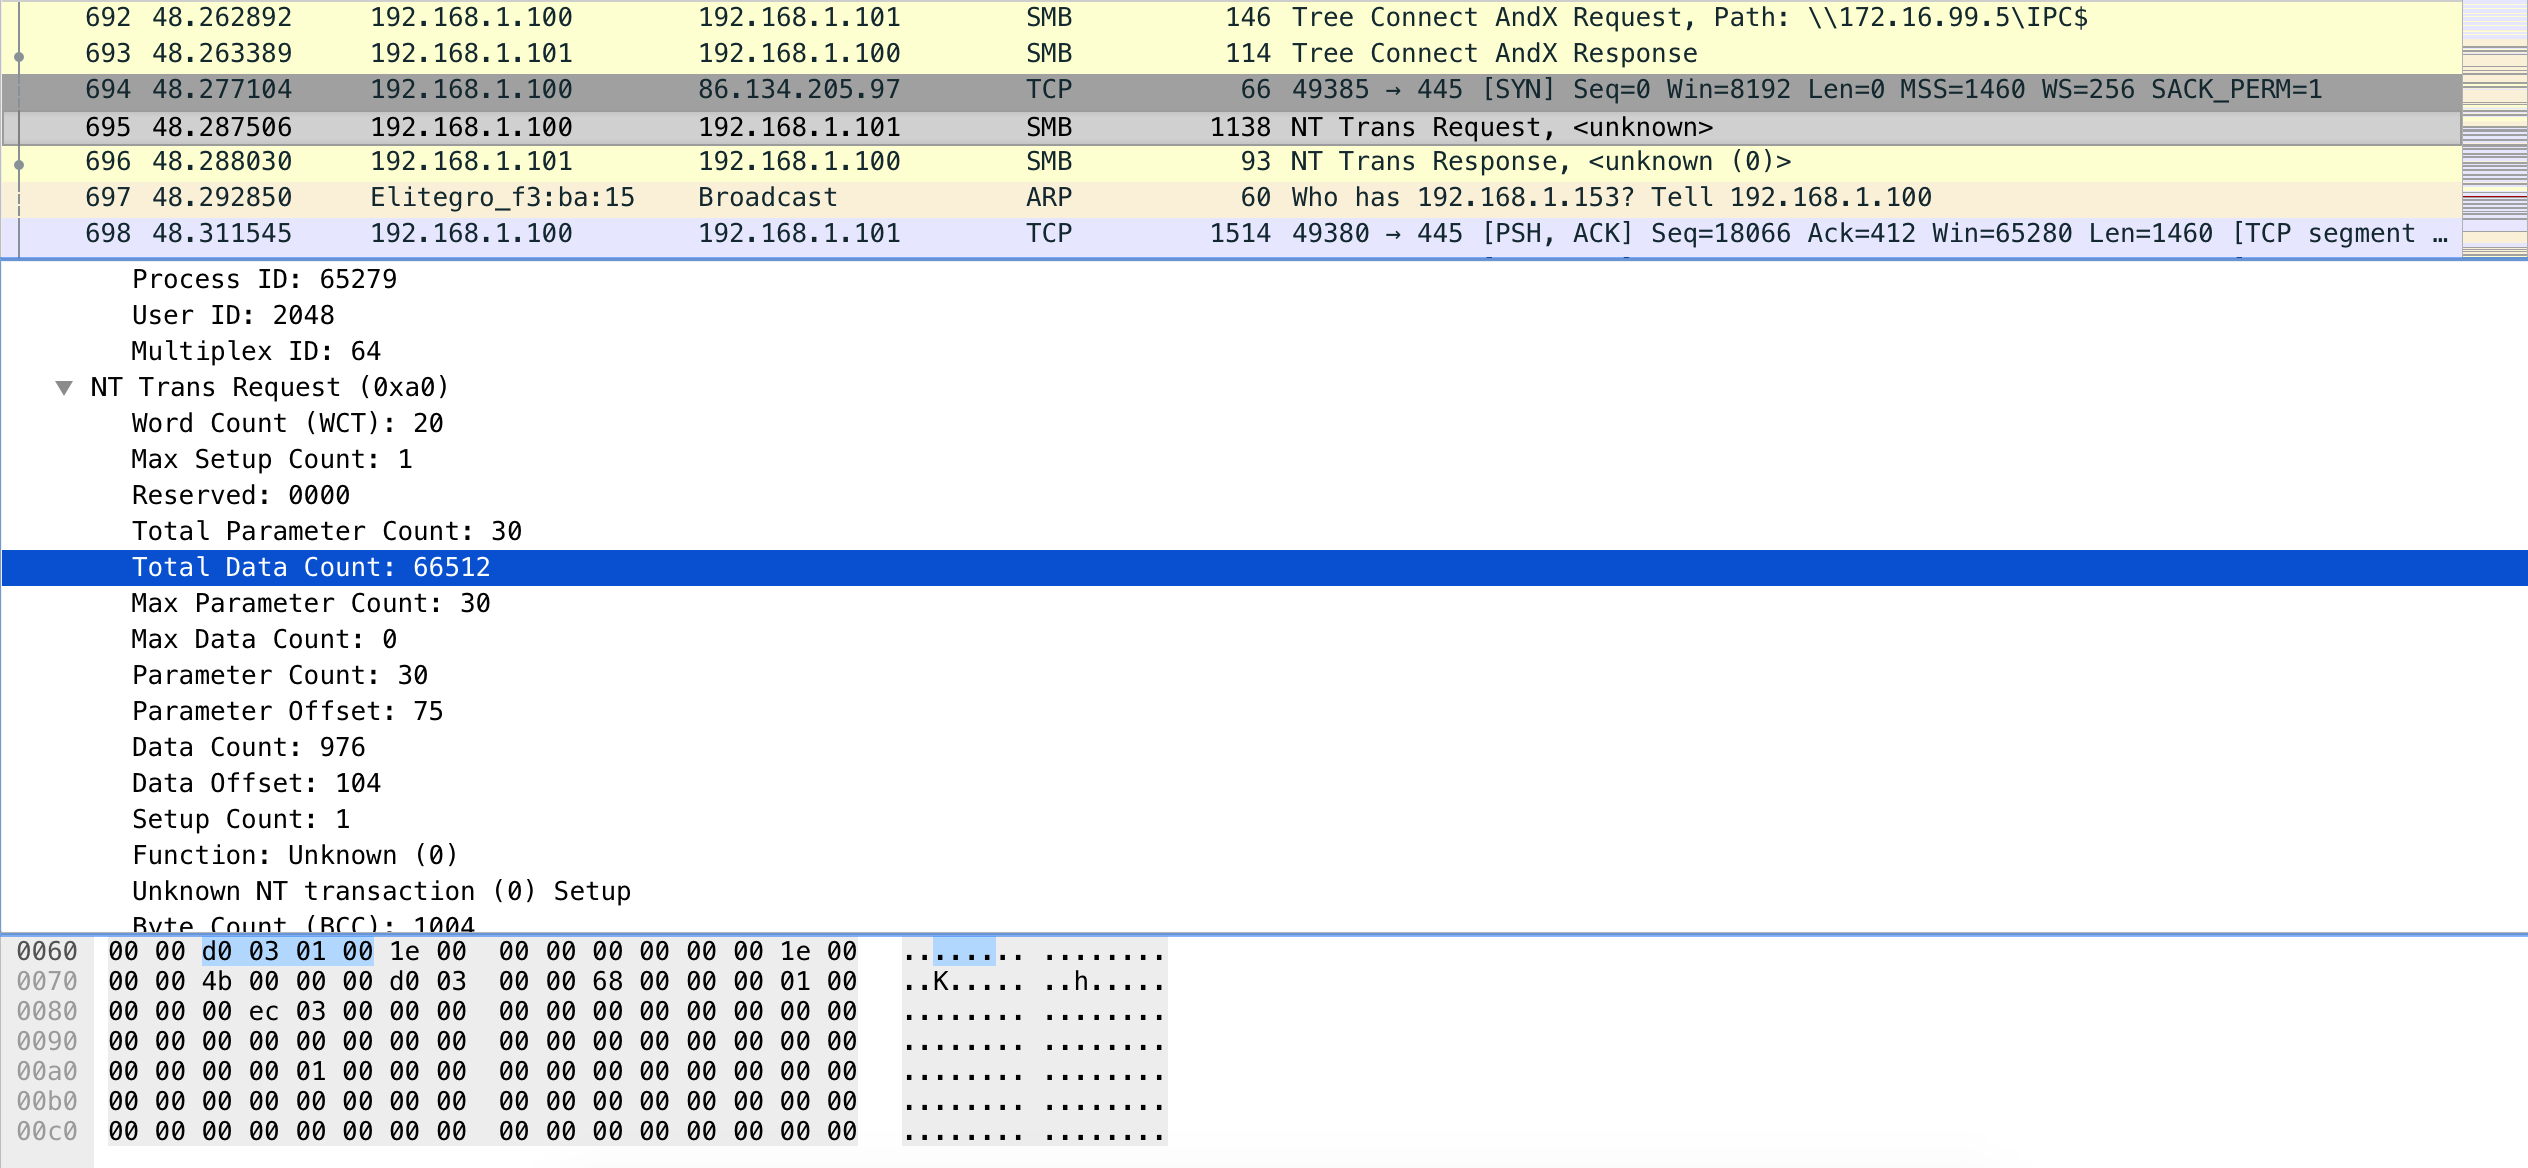
\includegraphics[width=\textwidth]{resources/trans_nop.png}
	\caption{Paket SMB\_COM\_NT\_TRANSACT dari host terinfeksi}
	\label{fig:trans_nop}
\end{figure}
\begin{figure}[H]
	\centering
	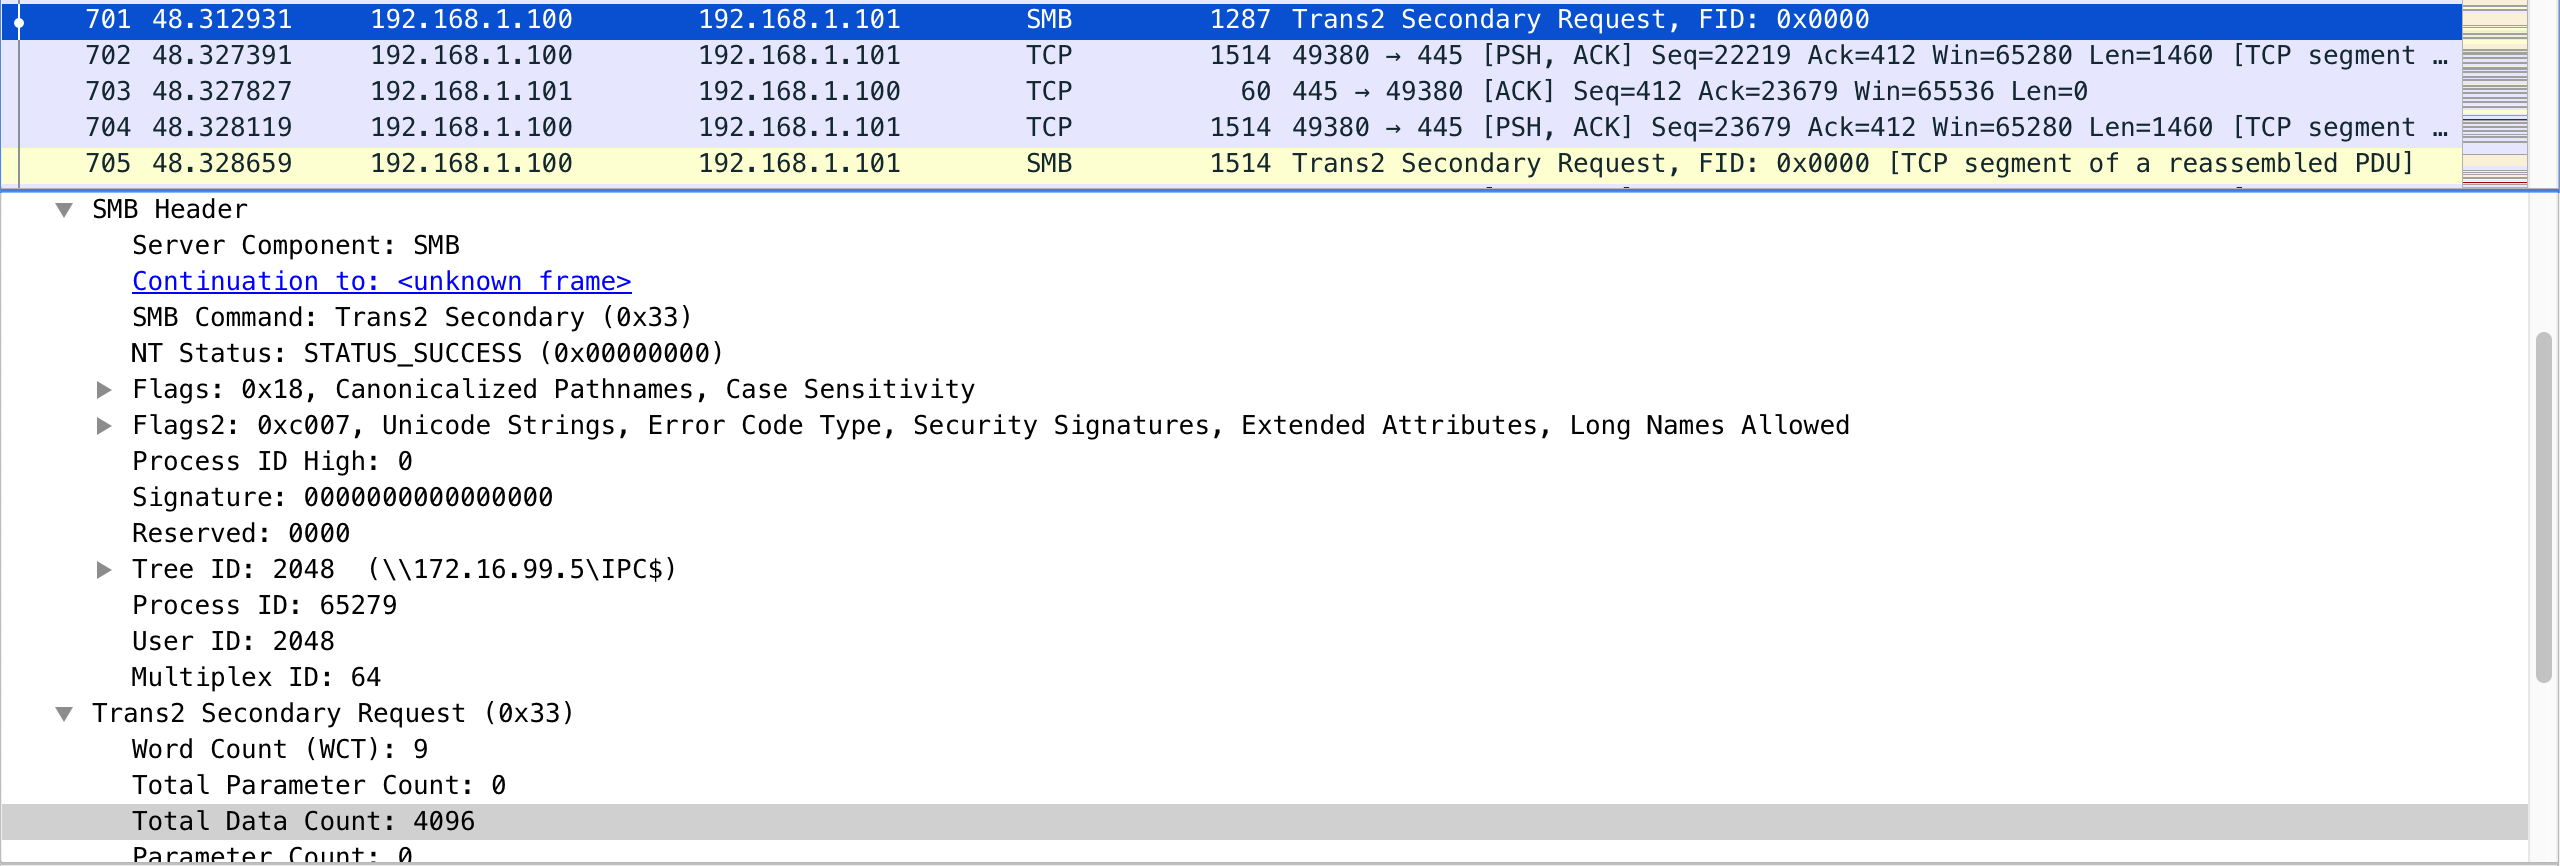
\includegraphics[width=\textwidth]{resources/trans2_secondary.png}
	\caption{Paket SMB\_COM\_TRANSACTION2\_SECONDARY dari host terinfeksi}
	\label{fig:trans2_secondary}
\end{figure}

Ketika payload sebuah perintah tidak cukup untuk dimasukkan ke dalam satu paket \verb|SMB_COM_NT_TRANSACT|, seharusnya kelebihan ini dimasukkan kedalam perintah \verb|SMB_COM_NT_TRANSACT_SECONDARY|. Tetapi WannaCry dengan sengaja menggunakan \verb|SMB_COM_TRANSACTION2_SECONDARY| sehingga menimbulkan \textit{wrong casting bug}. Kedua paket ini dapat dijadikan signature untuk deteksi ketika ada malware yang ingin melakukan eksploit terhadap vulnerability ini. Perlu sebuah kakas yang dapat mendeteksi jenis perintah yang digunakan oleh paket SMB.


\section{Analisis Kebutuhan}

Hasil analisis malware pada subbab sebelumnya untuk mencapai tujuan pada BAB I, diperlukan kakas yang dapat melakukan:

\subsection{Mekanisme Penangkalan Paket Malicious}

Ketika paket malicious dapat dideteksi, harus ada suatu mekanisme yang dapat menangkal paket tersebut sehingga tidak sampai ke host yang dituju. Pada konteks ini, firewall seharusnya dapat melakukan penangkalan agar paket \textit{malicious} dapat dihentikan.

Kakas yang umum digunakan untuk melakukan penangkalan paket dalam bentuk firewall pada sistem operasi linux adalah iptables. Iptables seperti dijelaskan pada subbab II.7 memiliki struktur umum yang dapat digunakan untuk berbagai keperluan. Penangkalan pada iptables dapat dilakukan dengan membuat aturan yang memiliki \textit{action} DROP atau REJECT.

\subsection{Deteksi Protokol Layer Aplikasi}

Penangkalan terhadap aktivitas \textit{malicious} terhadap host lain dapat dilakukan dengan mendeteksi signature yang terdapat pada paket yang dikirimkan. Untuk melakukannya, signature akan spesifik terhadap protokol layer aplikasi tertentu. Sehingga firewall harus dapat membedakan protokol yang digunakan pada layer aplikasi.

Deteksi jenis protokol layer aplikasi dapat dilakukan dengan menggunakan DPI seperti telah dibahas pada BAB II. Salah satu kakas yang umum digunakan adalah nDPI.

nDPI merupakan pengembangan OpenDPI (\cite{deri2014ndpi}). Jika dibandingkan dengan kakas lain, nDPI memiliki akurasi yang lebih tinggi seperti PACE, UPC MLA, dan Libprotoident (\cite{bujlow2013comparison}).

\subsection{State Machine}

Dari analisis malware yang telah dilakukan, untuk melakukan deteksi sebuah aktivitas \textit{malicious} dalam beberapa kasus tidak dapat ditentukan dari satu paket saja. Dalam kasus WannaCry dalam melakukan eksploitasi \textit{vulnerability} EternalBlue setidaknya perlu mendeteksi dua paket yakni \verb|SMB_COM_NT_TRANSACT| yang kemudian diikuti paket \verb|SMB_COM_TRANSACTION2_SECONDARY|.

Dengan menggunakan konsep state machine dan firewall yang melakukan pengecekan pada setiap paket, setiap paket dapat dikongruensikan sebagai alfabet pada state machine. Kemudian, bahasa yang diterima state machine merupakan semua aktivitas \textit{malicious} yang sesuai dengan signature.

\subsection{Deteksi Signature yang Paham terhadap Struktur Data}

Setelah diketahui jenis protokol yang digunakan, untuk dapat menangkal paket malicious seperti yang digunakan WannaCry untuk melakukan penyebaran, diperlukan sebuah kakas yang dapat mendeteksi paket yang dikirimkan sesuai dengan struktur data paket tersebut. Dengan melakukan pendeteksian yang memahami struktur data paket diharapkan dapat memperkecil kesalahan deteksi.

Namun, kakas deteksi seperti \verb|match string| hanya melakukan pencocokan pada payload dan tidak memiliki fitur untuk melakukan pencocokan pada bagian tertentu dari struktur data paket. Sehingga tidak dapat mendeteksi bagian seperti byte ke-n dari sebuah paket. Padahal hal ini diperlukan untuk melakukan pencocokan misalkan pada jenis perintah yang digunakan pada protokol SMB.

Berikut tabel \ref{table:software_requirement} yang merangkum kebutuhan perangkat lunak yang muncul untuk mencapai tujuan pada BAB I.

\begin{table}[H]
	\caption{Tabel kebutuhan perangkat lunak}
	\label{table:software_requirement}
	\begin{tabularx}{\textwidth}{|l|X|X|}
		\hline
		\textbf{No} & \textbf{Kebutuhan} & \textbf{Deskripsi} \\ \hline
		SR1 & Penangkalan paket & Perangkat lunak dapat menangkal sebuah paket ketika sebuah kondisi terpenuhi. \\ \hline 
		SR2 & State machine & Perangkat lunak dapat menyimpan dan merespon input berupa packet sehingga \textit{internal state} berubah. \\ \hline
		SR3 & Deteksi protokol level aplikasi & Perangkat lunak dapat mendeteksi protokol layer aplikasi. \\ \hline
		SR4 & Deteksi signature & Perangkat lunak dapat mendeteksi signature spesifik yang digunakan untuk melakukan eksploit vulnerability.\\ \hline
		SR5 & Menambahkan rule & Perangkat lunak dapat menerima masukan dari pengguna dalam bentuk aturan-aturan untuk perepresentasikan signature dari sebuah malware.\\ \hline
	\end{tabularx}
\end{table}

\section{Perancangan Sistem}

Perancangan dilakukan dengan menggunakan framework NetFilter. NetFilter merupakan framework native yang dimiliki oleh Linux untuk melakukan pemrosesan paket.


\subsection{Arsitektur Sistem}

Arsitektur sistem 

\subsection{Struktur Internal Sistem}

Dengan menggunakan framework netfilter, untuk membuat kakas analisis paket diperlukan \verb|xt_match| dan \verb|xtables_match| seperti pada diagram kelas \ref{fig:class_diagram}.

\begin{figure}[H]
	\centering
	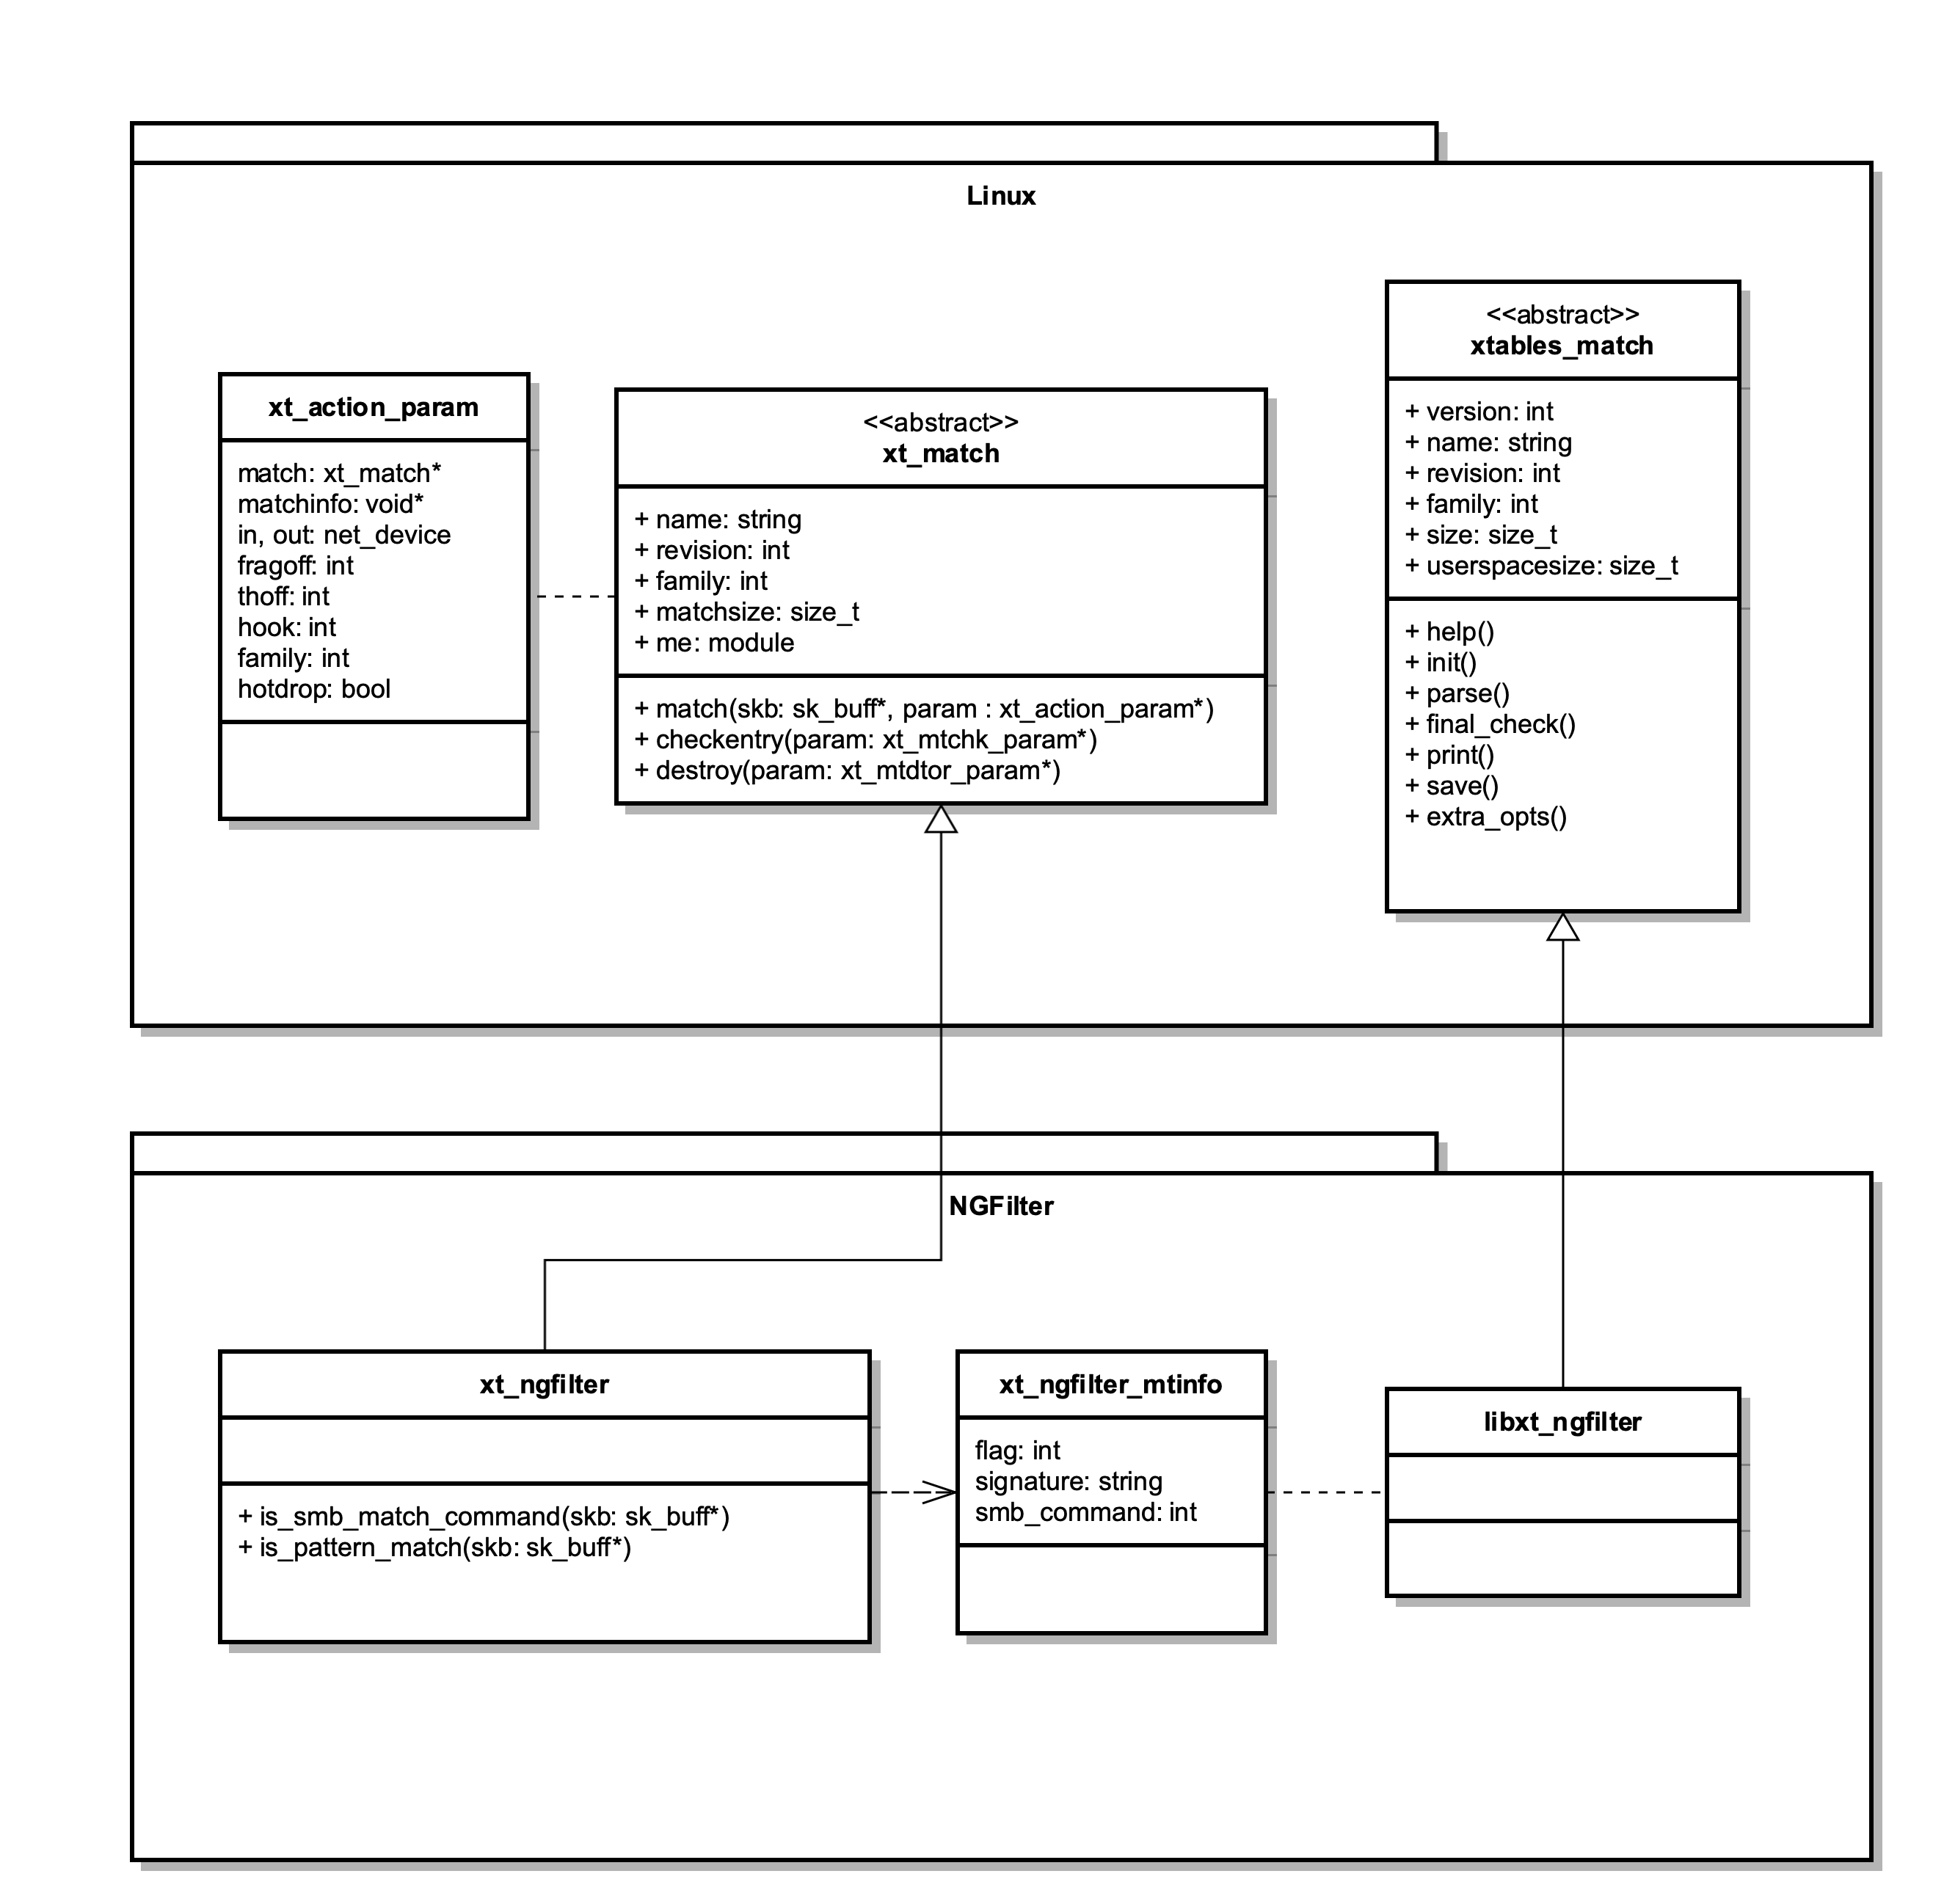
\includegraphics[width=\textwidth]{resources/ngfilter_class_diagram.png}
	\caption{Diagram Kelas}
	\label{fig:class_diagram}
\end{figure}

\verb|xtables_match| merupakan sebuah struct yang memiliki properti \verb|help|, \verb|init|, \verb|parse|, \verb|final_check|, \verb|print|, \verb|save|, \verb|extra_opts| yang merupakan method yang akan diinvoke ketika melakukan manipulasi terhadap rule iptables.

\verb|xt_match| merupakan sebuah struct yang memiliki properti \verb|match|, \verb|checkentry|, dan \verb|destroy| yang akan diinvoke pada kernel space ketika sebuah paket melewati hook dan kemudian melakukan match terhadap modul yang diimplementasi. Fungsi \verb|match| merupakan bagian yang menentukan apakah sebauh packet match dengan parameter-parameter yang ada pada rule.

\section{Perancangan State Machine dengan Iptables}



\section{Perancangan Rule dengan Iptables}

Rule akan diimplementasi dengan membuat sebuah state transition sebuah koneksi tcp. Hal ini dapat dilakukan dengan menggunakan modul mangle \verb|CONNTRACK|. State transition diagram \ref{fig:state_transition_diagram} menggunakan packet sebagai alfabet dan memiliki 3 state.

Seluruh koneksi pada awalnya berada pada state 0, dan akan terus pada state 0 hingga ditemukan signature bahwa koneksi merupakan koneksi SMB. Jika ditemukan signature, maka koneksi akan berubah menjadi state 1. Pada state 1 setiap paket akan dilakukan pengecekan terhadap command yang dilakukan. Jika ditemukan command \verb|COM_NT_TRANSACT| maka koneksi akan menjadi state 2. Kemudian state 2 ini merupakan state yang menentukan apakah ditemukan paket malicious yakni dengan mengirimkan \verb|COM_TRANSACTION2_SECONDARY| setelah \verb|COM_NT_TRANSACT|. Jika ditemukan maka koneksi akan ditandai untuk dilakukan \verb|DROP|.

\begin{figure}[H]
	\centering
	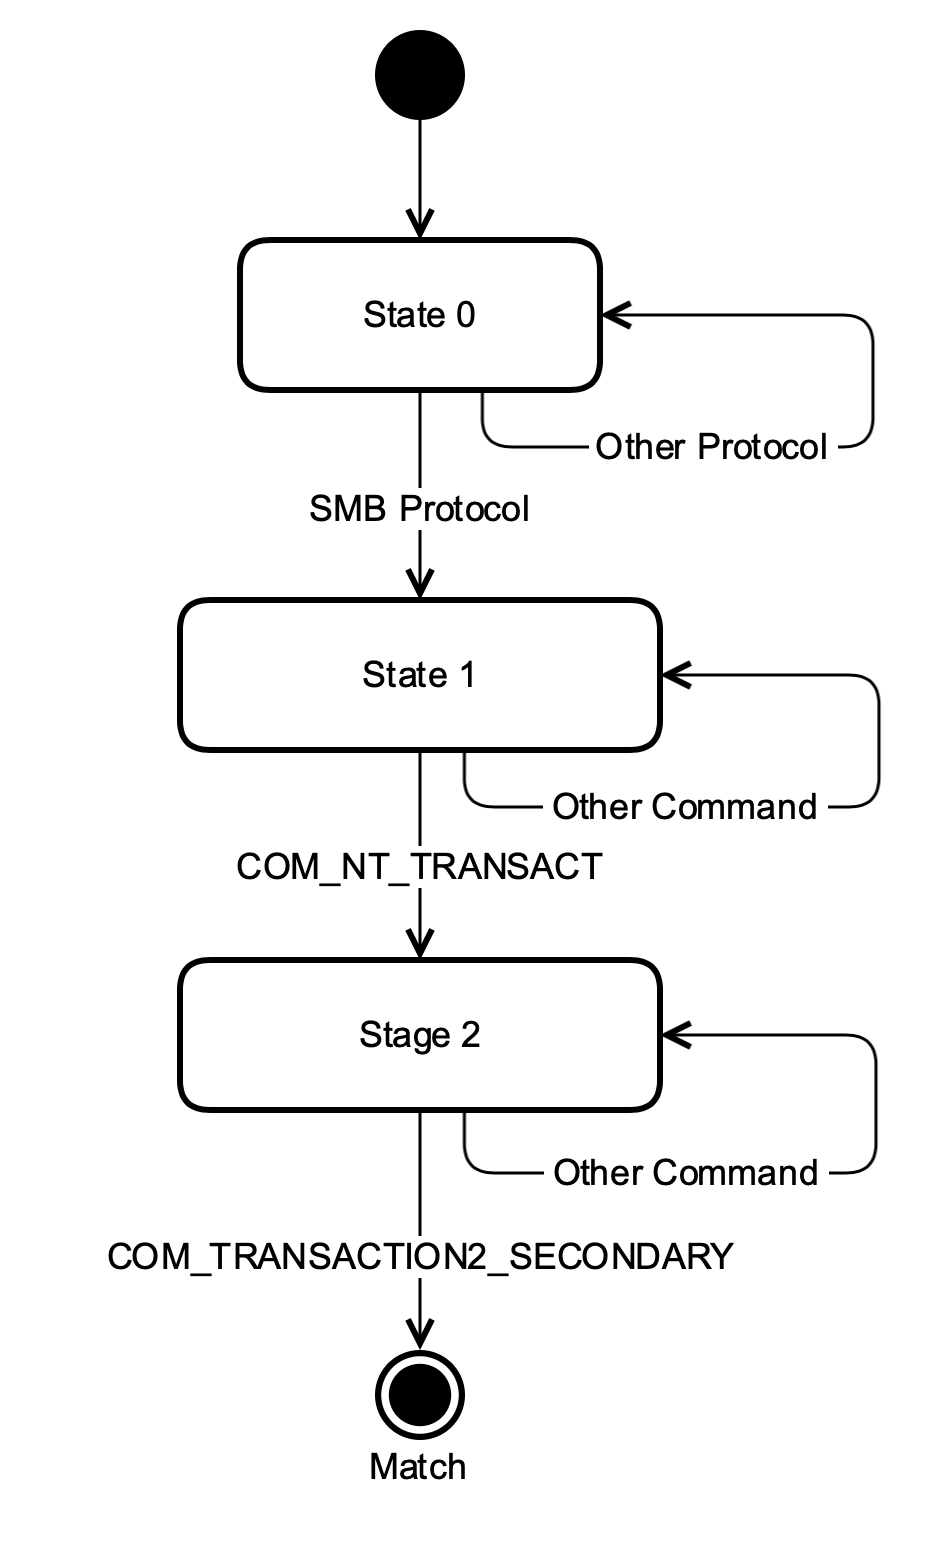
\includegraphics[width=200px]{resources/ngfilter_state_diagram.png}
	\caption{\textit{State Transition Diagram}}
	\label{fig:state_transition_diagram}
\end{figure}

\section{Traceability}

Pada tabel \ref{table:software_traceability_design} berikut ditunjukan kerunutan desain dan kebutuhan.

\begin{table}[H]
	\caption{Traceability perangkat lunak}
	\label{table:software_traceability_design}
	\begin{tabularx}{\textwidth}{|l|X|X|}
		\hline
		\textbf{No} & \textbf{Kebutuhan} & \textbf{Desain} \\ \hline
		SR1 & Penangkalan paket & menggunakan action DROP oleh iptables \\ \hline 
		SR2 & State machine &  menggunakan modul mangle \verb|CONNTRACK| \\ \hline
		SR3 & Deteksi protokol level aplikasi & menggunakan modul nDPI-NetFilter \\ \hline
		SR4 & Deteksi signature & class \verb|xt_ngfilter| pada diagram kelas \ref{fig:class_diagram} \\ \hline
		SR5 & Menambahkan rule & class \verb|libxt_ngfilter| pada diagram kelas \ref{fig:class_diagram} \\ \hline
 	\end{tabularx}
\end{table}
